\chapter{Information-Theoretic Arguments}
\setcounter{section}{-1}   % sections start at 11.0 (see main.tex comment)
\label{ch:inf}

\begin{objectives}
\item Recognize information-theoretic claims: content bounds (bits) or distinguishability bounds (divergence).
\item Prove the ladder: source coding $\to$ chain rule $\to$ KL/R\'enyi and Pinsker $\to$ incompressibility $\to$ Fano.
\item Match measure to task: entropy for space, KL for error, R\'enyi for composed stages, Fano for impossibility.
\item Dissect a paper's argument: random object, measure, chain-rule telescope, final bound.
\end{objectives}

Information theory counts information. Its two workhorses --- the \emph{entropy} of a
distribution (information content) and the \emph{divergence} between two distributions
(distinguishability) --- set limits no algorithm, protocol, or noise mechanism can
beat, in both directions. Downward: a quantity of $H$ bits can be written down in
about $H$ bits --- how sketches and compressible counters justify their footprint.
Upward: a task implicitly identifying one of $M$ objects forces $\log M$ bits --- how
space lower bounds and impossibility results are proved. Divergences do the same for
pairs: differential privacy \emph{is} a divergence bound between outputs on
neighboring inputs; a synthesizer's accuracy is a divergence to the truth.

In the SIGMOD'26 corpus the tool is tagged in a small cohort (5 papers) with a clean
division of labor: error bounds in three of the five (frequency-estimation sketching,
private query processing, private data-synthesis benchmarking), space lower bounds and
privacy guarantees in two each, and a PODS'26 entry that turns Shannon inequalities
directly into a join algorithm. Two exemplars (DP-S4S, Sublime) recur from
Chapters~\ref{ch:conc} and~\ref{ch:est}, but their information-theoretic side is a
different object from the side treated there. Section~\ref{sec:inf-advanced} adds
entropy as a difficulty measure, and further reading.

\section{The tool: information theory}

The problem class is uniform. Somewhere in the system there is a random object --- a
stream prefix, a pair of neighboring databases, a hypothesis about the data --- and the
question is not how a computation behaves \emph{on average} (Chapter~\ref{ch:conc}) but
how much \emph{information} the object carries, or how \emph{distinguishable} two of
its instantiations are. An entropy of $H$ bits is both a guarantee (an encoding of
length $\approx H$ exists) and a barrier (nothing shorter suffices).

\begin{remarkbox}[Notation]
Logs are base~2 (\emph{bits}) except for divergences $D$, $D_\alpha$, in \emph{nats}
(the divergence/privacy convention). $H(X)$: entropy of $X$; lowercase $h(X)$: the
\emph{entropy function} of a joint distribution viewed as a set function on attribute
sets (the join-processing usage). $p \ll q$: $q(x) = 0 \Rightarrow p(x) = 0$.
\end{remarkbox}

\subsection{The basic ladder}
\label{sec:inf-ladder}

\begin{definition}[Shannon entropy]\label{def:inf-entropy}
For a discrete random variable $X$ with distribution $p$, the \emph{entropy} is
\[
H(X) \;=\; -\sum_{x} p(x)\,\log_2 p(x) \qquad (0\log 0 := 0),
\]
and the \emph{conditional entropy} of $X$ given $Y$ is
$H(X \mid Y) = \sum_y \Pr[Y = y]\,H(X \mid Y = y)$. Entropy measures the number of bits
needed, on average, to pin down the value of $X$.
\end{definition}

The first rung makes that sentence a theorem \citep{information-theory-bg1,
information-theory-bg2}: no lossless code beats the entropy, and one within a bit
exists (``code'' = prefix-free binary description).

\begin{theorem}[Source-coding bound]\label{thm:inf-source}
Let $\ell\colon \mathcal{X} \to \mathbb{N}$ be the length function of any prefix-free
binary code for $X$. Then
\[
\mathbb{E}[\ell(X)] \;\ge\; H(X), \eopm
\]
with equality iff $\ell(x) = -\log_2 p(x)$. Conversely, the Shannon code $\ell(x) =
\lceil -\log_2 p(x)\rceil$ is prefix-free with $\mathbb{E}[\ell(X)] < H(X) + 1$.
\end{theorem}

\begin{proof}
Codewords are disjoint leaves of a binary tree, so Kraft's inequality gives
$Z := \sum_x 2^{-\ell(x)} \le 1$; set $q(x) = 2^{-\ell(x)}/Z$. Writing $D_2$ for the
KL divergence of Definition~\ref{def:inf-kl} in bits,
\[
D_2(p\|q) \;=\; \sum_x p \log_2\frac{p}{q}
\;=\; -H(X) + \mathbb{E}[\ell] + \log_2 Z \;\ge\; 0
\]
by Gibbs (Lemma~\ref{lem:inf-gibbs}); $\log_2 Z \le 0$ gives $\mathbb{E}[\ell] \ge
H(X)$, equality iff $q = p$, $Z = 1$. Conversely $\ell(x) = \lceil -\log_2 p(x)\rceil$
satisfies $2^{-\ell(x)} \le p(x)$, so Kraft holds, and $\ell < -\log_2 p + 1$.
\end{proof}

The second rung lets entropy telescope over multi-part objects --- the step that turns
a pipeline into an equation.

\begin{proposition}[Chain rule and conditioning]\label{prop:inf-chainrule}
For any pair of random variables,
\[
H(X,Y) \;=\; H(X) + H(Y \mid X),
\qquad\text{hence}\qquad
H(Y \mid X) \;\le\; H(Y),
\]
with equality in the second inequality iff $X$ and $Y$ are independent. \eop
\end{proposition}

\begin{proof}
Write $\log_2 p(x,y) = \log_2 p(x) + \log_2 p(y \mid x)$ and take $-\mathbb{E}$;
$H(Y|X) \le H(Y)$ follows by Jensen ($\log$ concave) over the average in $x$.
\end{proof}

The join-processing application needs the set-function form $h(X) = H(X)$, $X \subseteq
V$, for a joint distribution over variables $V$.

\begin{corollary}[Entropy is submodular; polymatroids]\label{cor:inf-submodular}
For all $X, Y, Z \subseteq V$:
\[
h(XY) + h(XZ) \;\ge\; h(X) + h(XYZ), \qquad h(XY) \ge h(X) \ge h(\emptyset) = 0.
\]
That is, the entropy function of any joint distribution is a \emph{polymatroid}
(normalized, monotone, submodular); inequalities valid for all polymatroids are called
\emph{Shannon inequalities}. \eop
\end{corollary}

\begin{proof}
$h(XY) + h(XZ) - h(XYZ) - h(X) = I(Y;Z \mid X) = H(Y|X) - H(Y|XZ) \ge 0$ by
Proposition~\ref{prop:inf-chainrule} applied twice; monotonicity is $H(Y|X) \ge 0$.
\end{proof}

The third rung measures distinguishability of two distributions
\citep{information-theory-bg2, information-theory-bg3}.

\begin{definition}[KL divergence]\label{def:inf-kl}
For distributions $p, q$ with $p \ll q$, the \emph{Kullback--Leibler divergence} is
\[
D(p \,\|\, q) \;=\; \sum_x p(x)\,\ln\frac{p(x)}{q(x)} \qquad (\text{nats}),
\]
and $D(p\|q) = \infty$ if $p \not\ll q$.
\end{definition}

\begin{lemma}[Gibbs]\label{lem:inf-gibbs}
$D(p\|q) \ge 0$ with equality iff $p = q$. \eop
\end{lemma}

\begin{proof}
$-D(p\|q) = \sum_x p(x)\ln\frac{q(x)}{p(x)} \le \ln\sum_x q(x) \le 0$ by Jensen
applied to the concave $\ln$ (the sum runs over $\operatorname{supp} p$).
\end{proof}

Two structural facts convert divergences along pipelines; both are one application of
the log-sum inequality \citep{information-theory-bg2} and both recur in the exemplars.

\begin{proposition}[Mixture convexity, chain rule, data processing]\label{prop:inf-klmix}
\leavevmode
\begin{enumerate}
\item (Convexity in the mixture.) If $P_i, Q_i$ are distributions and $\beta_i \ge
0$, $\sum_i \beta_i = 1$, then $D(\sum_i \beta_i P_i \,\|\, \sum_i \beta_i Q_i)
\le \sum_i \beta_i\,D(P_i \| Q_i)$.
\item (Chain rule.) With the same mixing distribution on both sides, the joint divergence
is the average of the conditional divergences:
\[
D(p(x)P(z|x) \,\|\, p(x)Q(z|x)) \;=\; \sum_x p(x)\,
D(P(\cdot|x) \,\|\, Q(\cdot|x)).
\]
Consequently
(data processing for a partition) $D(p\|q) \ge d(p(E) \| q(E))$ for every event $E$,
with $d$ the two-point divergence. \eop
\end{enumerate}
\end{proposition}

\begin{proof}[Proof sketch]
Expand $\sum_{x,z} p(x)P(z|x)\ln\frac{P(z|x)}{Q(z|x)}$: the $p(x)$ terms cancel,
giving (ii); (i) is the log-sum inequality applied per outcome. For the last claim,
let $z$ be the cell indicator of $E$ and drop the second, nonnegative term of (ii).
\end{proof}

Divergence controls total variation --- the bridge from information to probability:

\begin{theorem}[Pinsker]\label{thm:inf-pinsker}
For all $p, q$,
\[
\operatorname{TV}(p,q) \;:=\; \tfrac12 \sum_x |p(x) - q(x)| \;\le\;
\sqrt{\tfrac12 D(p\|q)}. \eopm
\]
\end{theorem}

\begin{proof}[Proof sketch]
Data processing (Proposition~\ref{prop:inf-klmix}) reduces to two points at the event
$E$ achieving total variation, $a = \Pr_p(E) > b = \Pr_q(E)$. The two-point divergence
has $\partial_b d(a\|b) = \frac{a-b}{b(1-b)}$, so $d(a\|b) = \int_b^a
\frac{a-t}{t(1-t)}\,dt \ge \int_b^a 4(a-t)\,dt = 2(a-b)^2$ since $t(1-t) \le
\tfrac14$: $D(p\|q) \ge 2\,\operatorname{TV}(p,q)^2$.
\end{proof}

The fourth rung parametrizes the divergence by an order $\alpha$ --- the calculus
privacy accounting runs on \citep{information-theory-bg3, information-theory-bg4}.

\begin{definition}[R\'enyi divergence]\label{def:inf-renyi}
For $\alpha \in (0,1) \cup (1,\infty)$,
\[
D_\alpha(p\|q) \;=\; \frac{1}{\alpha - 1}\,
\ln \sum_x p(x)^{\alpha}\, q(x)^{1-\alpha},
\]
with $D_1 = D(p\|q)$ (KL) and
$D_\infty = \ln\max_x \frac{p(x)}{q(x)}$ (\emph{max-divergence}).
\end{definition}

\begin{proposition}[R\'enyi calculus]\label{prop:inf-renyicalc}
$D_\alpha(p\|q)$ is nondecreasing in $\alpha$ (Figure~\ref{fig:inf-renyi}); $D_\infty$
is what pure differential privacy bounds, and every $\alpha > 1$ composes additively
\citep{information-theory-bg4, information-theory-bg5}. \eop
\end{proposition}

The mixture fact that survives the passage from KL to R\'enyi --- the engine of
Section~\ref{sec:inf-s4s} --- is quasi-convexity:

\begin{lemma}[Quasi-convexity of R\'enyi divergence; van Erven--Harremo\"es]\label{lem:inf-quasiconvex}
For any pairs $(P, Q)$, $(P', Q')$, any $0 < \beta < 1$, and $\alpha > 1$ (the case
privacy accounting uses),
\[
D_\alpha\bigl(\beta P + (1-\beta)P' \,\big\|\, \beta Q + (1-\beta)Q'\bigr)
\;\le\; \max\bigl\{ D_\alpha(P\|Q),\; D_\alpha(P'\|Q') \bigr\}. \eopm
\]
\end{lemma}

\begin{proof}
Let $F(r,s) = r^\alpha s^{1-\alpha}$ on $\mathbb{R}_+^2$: its Hessian has determinant
$0$ and positive diagonal entries, so $F$ is convex (linear along rays $s \propto r$).
Jensen applies outcome by outcome: $\sum_x (\beta p + (1-\beta)p')^\alpha(\beta q +
(1-\beta)q')^{1-\alpha} \le \beta A + (1-\beta)A' \le \max\{A, A'\}$, with
$A = \sum_x p^\alpha q^{1-\alpha} = e^{(\alpha-1)D_\alpha(P\|Q)}$, similarly $A'$;
dividing exponents by $\alpha - 1 > 0$ preserves the inequality.
\end{proof}

\begin{widefigure}[t]
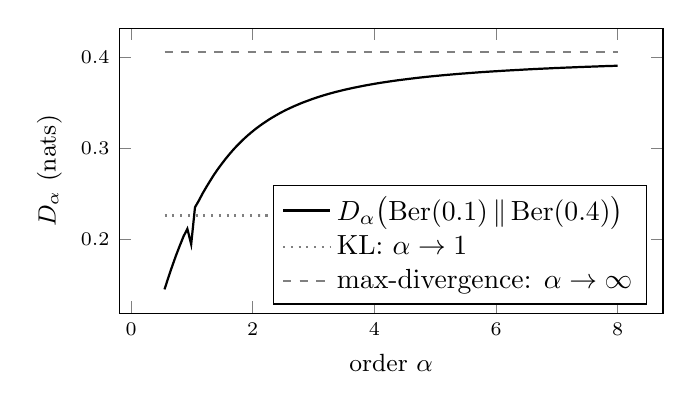
\begin{tikzpicture}
\begin{axis}[
  width=0.7\textwidth, height=5.2cm,
  xlabel={order $\alpha$}, ylabel={$D_\alpha$ (nats)},
  domain=0.55:8, samples=120,
  legend pos=south east, legend cell align=left,
  tick label style={font=\scriptsize}, label style={font=\small}
]
\addplot[black, thick]
  {ln(0.1^x * 0.4^(1-x) + 0.9^x * 0.6^(1-x))/(x-1)};
\addlegendentry{$D_\alpha\bigl(\mathrm{Ber}(0.1)\,\|\,\mathrm{Ber}(0.4)\bigr)$}
\addplot[gray, thick, dotted] {0*x + 0.2262};
\addlegendentry{KL: $\alpha \rightarrow 1$}
\addplot[gray, thick, dashed] {0*x + 0.4055};
\addlegendentry{max-divergence: $\alpha \rightarrow \infty$}
\end{axis}
\end{tikzpicture}
\caption{R\'enyi divergence vs.\ the order $\alpha$ for two Bernoulli distributions:
nondecreasing, through KL at $\alpha = 1$, converging to the max-divergence pure DP
bounds --- R\'enyi-DP certifies one point of this curve.}
\label{fig:inf-renyi}
\end{widefigure}

The last two rungs convert information into impossibility. First, incompressibility ---
the counting reading of Theorem~\ref{thm:inf-source}:

\begin{corollary}[Incompressibility]\label{cor:inf-counting}
If $X$ is uniform over $M$ outcomes then $H(X) = \log_2 M$, and any data structure
with $s$ bits that determines $X$ must satisfy $s \ge \log_2 M$: $s$ bits give fewer
than $2^s$ states, and each state witnesses only one $X$. \eop
\end{corollary}

\begin{proof}
Theorem~\ref{thm:inf-source} at the uniform distribution; the phrasing is pigeonhole.
\end{proof}

The method of \emph{incompressibility lower bounds} runs this backwards: too small a
sketch would be a code for objects of entropy beyond its bit count ---
Section~\ref{sec:inf-sublime} is a full exhibit. Second, Fano: an observation carrying
little information about a hypothesis pins down no estimator.

\begin{theorem}[Fano]\label{thm:inf-fano}
Let $X$ take $M \ge 2$ values, let $Y$ be generated through any channel from $X$, and
let $\hat X(Y)$ be any estimator. With $p_e = \Pr[\hat X(Y) \ne X]$,
\[
p_e \;\ge\; \frac{H(X \mid Y) - 1}{\log_2 M}. \eopm
\]
\end{theorem}

\begin{proof}[Proof sketch]
Condition on the error indicator $E = \mathbf{1}\{\hat X \ne X\}$: since $(X, E)$ is
determined by $(X, Y)$, $H(X|Y) \le H(E|Y) + H(X|E,Y) \le 1 + (1-p_e)\log_2 M$ ($E$
is binary; given $E = 0$, $X$ is determined by $Y$). Rearrange.
\end{proof}

\begin{corollary}[Capacity-style impossibility]\label{cor:inf-fano-cap}
If $X$ is uniform over $M$ hypotheses and the observable $Y$ satisfies $I(X;Y) =
\log_2 M - H(X|Y) \le c$, then every estimator errs with probability at least
$1 - (c+1)/\log_2 M$. \eop
\end{corollary}

\subsection{How to choose the information measure}
\label{sec:inf-choose}

The selection is mechanical once the deliverable is named. \emph{Space, communication,
or encoding bounds} ($\ge$ or $\approx$ bits): the source-coding pair
(Theorem~\ref{thm:inf-source}, Corollary~\ref{cor:inf-counting}) --- upper bounds by
exhibiting a code (Jensen bounds average code length), lower by incompressibility.
\emph{Distinguishability of two distributions} (privacy, testing, distributional
error): KL for expected-loss statements, R\'enyi $D_\alpha$ when stages compose ---
privacy accounting lives here, $\alpha$ tuned at the final conversion. \emph{Estimation
impossibility}: Fano (Theorem~\ref{thm:inf-fano}) with the capacity reading of
Corollary~\ref{cor:inf-fano-cap}. \emph{Structural size inequalities} (output sizes,
join costs): the Shannon-inequality system of Corollary~\ref{cor:inf-submodular},
optimized as a linear program.

\begin{reachbox}{When to Reach for Information Theory}
Reach when the claim is about \emph{information content} or
\emph{distinguishability} rather than average behavior: space lower bounds for
sketches, ``no mechanism can distinguish neighbors,'' ``no estimator recovers the
hidden data,'' ``this encoding is within $O(1)$ of optimal.'' Then run the recipe:
\begin{enumerate}
\item Name the random object: the stream prefix, the neighboring pair $(D, D')$, the
  hypothesis $X$ --- and what must be remembered, compared, or estimated about it.
\item Pick the measure: entropy for content (space/communication), KL for expected
  distributional error, R\'enyi $D_\alpha$ when stages compose (privacy accounting),
  Fano for estimation impossibility.
\item Write the chain-rule telescope along the structure: $H(X_1 \cdots X_k) = \sum_i
  H(X_i \mid \text{past})$, or the mixture decomposition over samples or stages.
\item Convert to the bound: $\mathbb{E}[\ell] \ge H$; $\operatorname{TV} \le
  \sqrt{D/2}$; $p_e \ge (H(X|Y)-1)/\log M$ (Fano); $\varepsilon' = \varepsilon +
  \ln(1/\delta)/(\alpha-1)$ (privacy conversion).
\end{enumerate}
\end{reachbox}

\section{Shannon inequalities as a join algorithm}
\label{sec:inf-panda}

The exemplar is a PODS'26 paper on join query processing \citep{sigmod26-185}\pods.
Evaluating conjunctive queries is the heart of database theory, and worst-case optimal
algorithms alone ignore the \emph{skew} real data exhibits: a degree constraint saying
``each value of $X$ has at most $N_{Y|X}$ matching $Y$s'' can shrink the output by
orders of magnitude. The PANDA framework exploits such constraints through the
polymatroid inequalities of Corollary~\ref{cor:inf-submodular}, but the original
algorithm pays for its generality with complex recursive partitioning. The paper
introduces \emph{PANDAExpress}: pick the inequality's weights by LP duality, and turn
each Shannon-inequality proof step into a recursive hyperplane partition of the data.
The result computes a query model meeting the polymatroid size bound $B$ in time
$O(N \log N + B \log N)$, recovering fractional hypertree-width and submodular-width
runtimes as corollaries.

\paragraph{Problem.}
Queries are \emph{disjunctive datalog rules} (DDRs)
\[
Q(Z) \;:\!-\; \bigvee_{R(X) \in \Sigma_{\mathrm{in}}} R(X)
\]
An output \emph{model} assigns tuples to the atoms
$Q(Z) \in \Sigma_{\mathrm{out}}$ so that every tuple $t$ of the natural join
$\Join_{\Sigma_{\mathrm{in}}}$ is covered, i.e.\ $t_Z \in Q(Z)$ for some $Z$; the goal
is a \emph{small} model. The instance satisfies \emph{degree constraints}
$(\Delta, N)$: for each term $\delta = (Y|X) \in \Delta$, the max degree
$\deg_R(Y|X{=}x)$ is at most $N_\delta$ in some input relation $R$. Writing $h$ for
the entropy function of any distribution consistent with the constraints, a
\emph{Shannon-flow inequality} is
\[
\sum_{Z \in \Sigma_{\mathrm{out}}} \lambda_Z\, h(Z) \;\le\;
\sum_{\delta \in \Delta} w_\delta\, h(\delta),
\qquad \| \lambda \|_1 = 1, \ \ \lambda, w \ge 0 \ \text{rational},
\]
valid for all polymatroids, where $h(Y|X) = h(XY) - h(X)$; it certifies
$|\Sigma_{\mathrm{out}}| \le B$ with $B = \prod_\delta N_\delta^{w_\delta}$ (take
logs of $h(\delta) \le \log N_\delta$).

\paragraph{Guarantee.}

\begin{theorem}[PANDAExpress, Theorem~6.4 of the paper]\label{thm:inf-panda-main}
Given a DDR, an input instance over $\Sigma_{\mathrm{in}}$ of size $N$ satisfying
degree constraints $(\Delta, N)$, and a Shannon-flow inequality with weights
$(\lambda, w)$, PANDAExpress computes a model $\Sigma_{\mathrm{out}}$ for the DDR of
size
\[
\|\Sigma_{\mathrm{out}}\| \;=\; O(B)
\quad\text{in time}\quad
O\bigl(N\log N + B\log N\bigr),
\qquad B \;=\; \prod_{\delta\in\Delta} N_\delta^{w_\delta}. \eopm
\]
\end{theorem}

\paragraph{How information theory is applied.}
Everything hangs on one move: the paper gives the Shannon inequality a
\emph{measure-theoretic} second life. A sub-probability measure is a nonnegative
function with total mass at most $1$; its marginals and conditionals are again such,
and so is the geometric mean of $k$ of them (AM--GM/H\"older on the masses). The
weights come first: LP duality (Proposition~6.3 of the paper) minimizes
$B = \prod_\delta N_\delta^{w_\delta}$ subject to the Shannon-flow inequality, and any
optimal solution puts $w_\delta = 0$ on every constraint with $N_\delta > B$: the
budget ignores loose constraints. The workhorse then converts the inequality into
measures: instantiate each constraint $\delta = (Y|X)$ on the data as
$p_\delta(y|x) = 1/N_\delta$ if $(x,y)$ occurs in some input relation, $0$ otherwise
--- a sub-probability conditional.

\begin{lemma}[Measures from inequalities; Lemma~4.4 of the paper, notation cleaned]
\label{lem:inf-panda-measures}
Let $(\lambda, w)$, $\|\lambda\|_1 = 1$, be nonnegative rational weights for which
$\sum_Z \lambda_Z h(Z) \le \sum_\delta w_\delta h(\delta)$ is a Shannon-flow inequality
over $V$. Then for any collection of sub-probability measures $p_\delta$, $\delta \in
\Delta$, there exist sub-probability measures $p_Z$, $Z \in \Sigma_{\mathrm{out}}$,
such that
\[
\prod_{Z \in \Sigma_{\mathrm{out}}} p_Z(t)^{\lambda_Z} \;\ge\;
\prod_{\delta \in \Delta} p_\delta(t)^{w_\delta}
\qquad \text{for all } t \in \mathrm{Dom}_V. \eopm
\]
\end{lemma}

\begin{proof}[Proof sketch]
Clear denominators to an \emph{integral} Shannon-flow inequality over multisets; it
has a \emph{proof sequence} (Theorem~2.4 of the paper): single steps of submodularity,
composition, decomposition, or monotonicity. Give each term of $\mathcal{D}$ its
measure; at every step replace measures so the pointwise product only grows:
monotonicity $h(XY) \to h(X)$ replaces $p_{XY}$ by its marginal; submodularity
$h(Y|X) \to h(Y|XZ)$ re-conditions, $p_{Y|XZ}(y|xz) := p_{Y|X}(y|x)$; composition and
decomposition split $p_{XY} = p_X \cdot p_{Y|X}$ or merge back. The final multiset
contains $\mathcal{Z}$; group equal terms by geometric means (still sub-probability)
and normalize exponents back to $(\lambda, w)$. Full case analysis in
Section~\ref{sec:inf-appendix}.
\end{proof}

The bound follows by ``taking logs'': for a join tuple $t \in
\Join_{\Sigma_{\mathrm{in}}}$, every $p_\delta(t) = 1/N_\delta$, so the right-hand
product is $1/B$; since $\|\lambda\|_1 = 1$, some $Z$ has $p_Z(t_Z) \ge 1/B$, and the
model $Q(Z) = \{z : p_Z(z) \ge 1/B\}$ covers every join tuple and has at most $B$
tuples because $p_Z$ has mass $\le 1$ --- Markov at the measure level.
\sidenote{Why \emph{hyperplanes}: no axis-parallel light/heavy split proves one
two-atom cover, but the tilted hyperplane $h(C) = h(F)$ does; the geometric-mean
construction finds such cuts automatically.} The algorithm
implements each proof step as a recursive partition along the step's measure threshold
(light tuples continue the proof sequence; the heavy side restarts via the paper's
Reset Lemma), and a potential $|\mathcal{D}| + |\mathcal{M}| + 3|\mathcal{S}|$
decreases at every restart, bounding the recursion depth by the proof length.

\paragraph{What it buys.}
Worst-case-optimal evaluation \emph{with} skew at $O(N\log N + B\log N)$, where prior
PANDA-style algorithms needed many bucket partitions per cut --- and the theory
delivers the algorithm, not just the bound: each proof step is executable.

\section{R\'enyi-divergence accounting for sampled private queries}
\label{sec:inf-s4s}

The exemplar is a SIGMOD'26 paper on private query processing \citep{sigmod26-079}.
Answering select--join--aggregate (SJA) queries under \emph{user-level} differential
privacy --- no adversary may confidently infer the presence or absence of any one
\emph{user's} entire tuple set --- is demanding, because users contribute unboundedly
many tuples and one heavy user can dominate the answer, and the state of the art
attains strong accuracy only via expensive optimization over the whole database. The
paper's engine, DP-S4S, accelerates the search by Poisson-sampling tuples before
privatizing, truncates each heavy user's contribution at a threshold found privately
by a sparse-vector-technique (SVT) search, and releases through a smooth-sensitivity
Gaussian mechanism. Its privacy analysis is pure
information theory: privacy \emph{is} a divergence bound between neighboring outputs,
sampling turns each output into a \emph{mixture} over samples, and the divergence of
mixtures is controlled by R\'enyi quasi-convexity, with a binomial count deciding
which components matter.

\paragraph{Problem.}
Privacy of a mechanism $M$ is a bound on how distinguishable $M(D)$ and $M(D')$ are for
\emph{neighboring} inputs $D \sim D'$ (user-level: all tuples of one user added or
removed). The information-theoretic formulation used here is R\'enyi differential
privacy \citep{information-theory-bg5}:

\begin{definition}[R\'enyi DP, user level]\label{def:inf-rdp}
For $\alpha > 1$ and $\varepsilon > 0$, a randomized mechanism $M$ is
$(\alpha, \varepsilon)$-RDP if for all neighboring $D, D'$,
\[
D_\alpha\bigl(M(D) \,\big\|\, M(D')\bigr) \;\le\; \varepsilon,
\]
with $D_\alpha$ as in Definition~\ref{def:inf-renyi}. An $(\infty, \varepsilon)$
bound is pure $\varepsilon$-DP; RDP converts back to
$(\varepsilon + \frac{\ln(1/\delta)}{\alpha - 1},\, \delta)$-DP for any $\delta > 0$.
\end{definition}

The engine Poisson-samples each tuple independently with probability $q$ (sample
$S \subset T$), runs an SVT search $M_1$ over truncation thresholds on $S$, and
releases the truncated aggregate through a Gaussian mechanism $M_2$ calibrated in
R\'enyi terms. The pipeline is $L = \ell + 1$ stages ($\ell$ SVT iterations plus the
release), each needing an amplified budget: sampling shrinks the effective
divergence, and the analysis must say by how much.

\paragraph{Guarantee.}

\begin{corollary}[RDP-S4S for scalar SJA; Corollary of the paper, notation cleaned]
\label{cor:inf-s4s-rdp}
There is an $(\alpha, \varepsilon)$-RDP version of the engine's main algorithm. Let $n$
be the number of records, $m$ the number of users, $q$ the sample rate,
$\tau^*(T) = \max_u \sum_{t \in T}\mathbf{1}[u \prec t]$ the maximum per-user
contribution, and $\varepsilon_i^* \ge \varepsilon/(\ell+1)$ the amplified
noise-calibration budget. With probability $1 - \beta$,
\[
\bigl|\hat f(T) - f(T)\bigr|
\;=\; O\Bigl(\sqrt{\tfrac{n}{q}} + \tfrac{1}{q} +
\frac{\sqrt{\alpha}}{\varepsilon_i^*}\Bigl(\tau^*(T) + \sqrt{\tfrac{\tau^*(T)}{q}}\Bigr)\Bigr),
\]
where $O(\cdot)$ hides constants and polylogarithmic factors in $m$ and $1/\beta$. \eop
\end{corollary}

\paragraph{How information theory is applied.}
The random object is the pair of \emph{output distributions on neighboring inputs} ---
and sampling makes each a mixture:
$\Pr[M(T) = z] = \sum_S \Pr[\lambda(T){=}S]\cdot\Pr[M(S) = z]$. Quasi-convexity
(Lemma~\ref{lem:inf-quasiconvex}) bounds the mixture's divergence by the worst
component, $D_\alpha\bigl(\sum_S p_S M(S) \,\|\, \sum_S p_S M(S \cup S_u)\bigr) \le
\max_S D_\alpha(M(S) \| M(S \cup S_u))$; the reverse direction uses convexity in the
second argument plus concavity of $\ln$ (the Proposition~\ref{prop:inf-klmix} logic,
order by order). The per-component divergence is Gaussian, closed-form:

\begin{lemma}[Gaussian R\'enyi divergence; Lemma of the paper, notation cleaned]
\label{lem:inf-gauss-renyi}
For $\mu_1, \mu_2 \in \mathbb{R}^d$ and i.i.d.\ noise,
\begin{align*}
D_\alpha\bigl(\mathcal{N}(\mu_1, \sigma_1^2 I_d) \,\|\, \mathcal{N}(\mu_2, \sigma_2^2
I_d)\bigr)
\;&=\; \frac{\alpha \,\|\mu_1 - \mu_2\|_2^2}{2\sigma^2_\mathrm{mix}}\\
\;&+\; \frac{d}{2}\,(\alpha - 1)\,
\ln \frac{\sigma_1^{\,2(1-\alpha)}\,\sigma_2^{\,2\alpha}}{\sigma^2_\mathrm{mix}},
\eopm
\end{align*}
where $\sigma^2_\mathrm{mix} = (1-\alpha)\sigma_1^2 + \alpha\sigma_2^2$; the
divergence is infinite if $\sigma^2_\mathrm{mix} \le 0$. For equal scales $\sigma$,
only the first term survives: $D_\alpha = \alpha\|\mu_1 - \mu_2\|_2^2 / 2\sigma^2$.
\end{lemma}

The count structure now enters: user $u$ contributes $k$ of its $\hat\tau$ sampled
tuples to $S \cup S_u$ with probability $p_k = \Pr[\mathrm{Bin}(\hat\tau, q) = k]$, and
the truncated query moves by at most $\min\{\tau, k\}$ between components --- the
amplified budget is a binomial average of per-count Gaussian divergences,
$\varepsilon'(\alpha) = \frac{1}{\alpha-1}\ln\bigl(\sum_{k \le \hat\tau} p_k
\exp((\alpha-1)\, c\,\min\{\tau,k\}^2) + \Pr[\mathrm{Bin}(\hat\tau,q) > \hat\tau]\,
e^{(\alpha-1)\varepsilon_s}\bigr)$ with $c$ set by the noise scale (``RDP
Amplification'' Lemma of the paper; some symbols dropped by the extractor, structure
preserved). In the pure-DP limit this yields
$\varepsilon' = \ln\bigl(1 + q'(e^{\varepsilon_1} - 1)\bigr)$ with
$q' = 1 - (1-q)^{\hat\tau}$ --- subsampling amplification with the collision
probability $q'$ in place of $q$. Finally the stages compose: RDP composition sums the
$L$ budgets (Proposition~\ref{prop:inf-renyicalc}), and Definition~\ref{def:inf-rdp}'s
conversion returns to $(\varepsilon, \delta)$-DP, $\alpha$ chosen once to optimize the
final $\varepsilon$.

\paragraph{What it buys.}
User-level privacy whose accounting survives $L$-stage composition without the
$\sqrt{L}$ loss of naive advanced composition, sampling amplification recognized as a
divergence shrink, and --- via the $\sqrt{\alpha}$ term in
Corollary~\ref{cor:inf-s4s-rdp} --- a dial trading R\'enyi order against noise scale.

\section[Source coding for expandable sketches]{Source coding and incompressibility for expandable sketches}
\label{sec:inf-sublime}

The exemplar is a SIGMOD'26 paper on streaming frequency estimation
\citep{sigmod26-231}, read here through the entropy lens rather than the estimator
lens of Chapter~\ref{ch:est}. Frequency-estimation (FE) sketches such as Count-Min and
CountSketch commit to a fixed width at construction, but real streams are unbounded
and skewed: the length is unknown in advance, heavy keys make some counters grow
large while most stay tiny. The paper's system, \emph{Sublime}, is an expandable
CountSketch-style sketch that grows with the stream, and its two-sided theory is a
textbook information argument. Upper bound, source coding: counters are stored as
short stubs plus rare extensions, and Jensen (concavity of $\log$) shows the array
encodes in about $w \log_2(k/w) + O(w)$ bits --- within a constant of the information
content of $w$ counters summing to $k$. Lower bound, incompressibility: any FE sketch
achieving error $E(N)$ at confidence $1-\delta$ on growing streams must at some point
hold at least $\frac{N}{E(N)}\bigl[\Omega(\log \frac1\delta +
\log\log\frac{N}{E(N)}) - \Theta(1)\bigr]$ bits, else its state would compress random
key sequences below their entropy.

\paragraph{Problem.}
A stream of keys (insertions, deletions) of unknown ultimate length $N$ is processed
by an \emph{expandable} FE sketch maintaining $d$ counter arrays whose width follows a
size function $W(\cdot)$ --- e.g.\ $W(N) = N/\varepsilon$ or $W(N) =
N^\alpha/\varepsilon$ with $0 \le \alpha < 1$ --- expanding over \emph{epochs} at
width $W_j = W(N_j)$. Skew makes the counter values far from uniform: a few large,
many small, and the storage cost depends on how compactly that multiset is
\emph{written down}. The lower-bound adversary is any FE sketch with only
overestimation errors guaranteeing error $E(N)$ at confidence $1-\delta$ on a
growing stream.

\paragraph{Guarantee.}

\begin{theorem}[Memory footprint; Theorem of the paper, notation cleaned]
\label{thm:inf-sublime-space}
With a sublinear power size function, the sketch's memory footprint is
\[
\approx \;d \cdot W(N) \cdot \bigl[4.41 + 1.26\cdot \log_2 \tfrac{N}{W(N)}\bigr]
\ \text{bits};
\]
with a linear size function, $\approx d \cdot W(N) \cdot [4.41 + 1.26\log_2
\frac{N\log_2 N}{W(N)}]$. The same bounds hold with $W(F)$ (the squared $\ell_2$ norm)
in place of $W(N)$, plus one bit per counter if counters are signed. \eop
\end{theorem}

\begin{theorem}[Space lower bound; Theorem of the paper]\label{thm:inf-sublime-lb}
Any FE sketch with only overestimation errors that processes growing streams with error
bound $E(N)$ and confidence $1-\delta$ must use at least
\[
\frac{N}{E(N)}\cdot\Bigl[\Omega\Bigl(\log\tfrac{1}{\delta} +
\log\log\tfrac{N}{E(N)}\Bigr) - \Theta(1)\Bigr] \eopm
\]
bits of memory at some point in time while processing a stream.
\end{theorem}

\paragraph{How information theory is applied.}
The upper bound runs the source-coding direction of Theorem~\ref{thm:inf-source}. A
single counter value $v$ is coded as an $s$-bit \emph{stub} plus, when $v \ge 2^s$, a
variable-length \emph{extension} of $\lfloor v/2^s \rfloor$ in base $3$ --- at most
$4 + 1.26\log_2 v$ bits in total (Lemma of the paper; the constant $1.26 =
2\log_3 2$ is the base conversion). The array-level step is the entropy-flavored one:

\begin{lemma}[Counter-array encoding; Lemma of the paper, notation cleaned]
\label{lem:inf-sublime-array}
An array of $w$ unsigned counters with total absolute value $k$ encodes in
\[
w\cdot\bigl[4.41 + 1.26\cdot\log_2 (k/w)\bigr] \ \text{bits}, \eopm
\]
and signed counters cost one extra bit each.
\end{lemma}

\begin{proof}[Proof sketch]
Sum the per-counter bound and use the concavity of $\log_2$ \emph{twice}: the stub
length satisfies $s \le 2 + \frac1w\sum_i \log_2|v_i| \le 2 + \log_2(k/w)$ (Jensen),
and after replacing each per-counter term by the larger of the two scales,
$\sum_i \log_2(\frac{k}{4w} + |v_i|) \le w\log_2(\frac54 \cdot \frac kw)$ (Jensen
again); $1.26\log_2\frac54 \approx 0.41$ supplies the constant. Full proof in
Section~\ref{sec:inf-appendix}.
\end{proof}

The lower bound runs the converse, Corollary~\ref{cor:inf-counting}, as a
\emph{reduction to compression}: a smaller sketch would compress sequences $\bar x =
(x_1, \dots, x_n)$ of $n = N/(2E(N))$ keys drawn uniformly from a universe of size
$u \cdot n$ --- objects of entropy $n\log_2(un)$. Three steps. First, a
\emph{variance chain rule} (law of total variance over the sketch's estimates across
prefixes $\bar x_1, \dots, \bar x_\ell$ of geometrically growing lengths) exhibits
one prefix state $\mathcal{S}^*_i$ whose estimates have second moment at most
$2V/\log_2 n$. Second, \emph{fixing the internal randomness}: averaging over the seed
makes bias and variance small simultaneously, so one seed works on at least half of
all sequences --- a seed with $\mu(\bar x) \le 64\delta/\log_2 n$ and $\nu(\bar x)
\le 64\delta/\log_2 n$ on at least half the sequences (Lemma of the paper). Third,
the \emph{code}: write $\bar x$ as (seed, state of $\mathcal{S}^*_i$); a decoder
re-queries the sketch for every key and recovers $\bar x$ up to the error event, so
the codewords are nearly injective over half of a set of entropy $n\log_2(un)$. The
state must hold $n\log_2(un) - O(n \cdot E(N))$ bits minus the seed index, which
unwinds to the stated $\frac{N}{E(N)}[\log \frac1\delta + \log\log \frac{N}{E(N)} -
\Theta(1)]$: a sketch that answers queries is a code.

\paragraph{What it buys.}
A footprint certified \emph{while it grows} --- no prior knowledge of stream length
or skew --- within a small logarithmic factor of what any expandable FE sketch must
pay; the same entropy accounting compresses its counters and fences off its
competition.

\section{Divergence budgets for private data synthesis}
\label{sec:inf-dpsynth}

The exemplar is a SIGMOD'26 Experiments \& Analysis paper benchmarking differentially
private tabular data synthesis \citep{sigmod26-279}. A DP synthesizer generates a fake
table preserving useful statistics of a real one while protecting every individual's
row; synthesizers are pipelines --- select marginals, discretize, infuse noise,
compose the joint --- and competing systems make incomparable accuracy/privacy
choices, so evaluations are hard to interpret. The paper benchmarks representative
synthesizers under a unified treatment: every stage's privacy loss is an
$(\alpha, \varepsilon)$-RDP budget, stages compose additively, and accuracy is the
\emph{KL divergence} between synthesized and true joint. Its theory contribution is
an ordering theorem: estimating a joint through noisy \emph{conditionals} is never
worse in KL error than a \emph{product of noisy marginals} --- the divergence version
of ``conditionals carry the dependence.'' The extract records the statements without
proofs; we transcribe conservatively and flag where the standard argument fills in.

\paragraph{Problem.}
The pipeline is a composition of randomized stages over a table with attributes
$A_1, \dots, A_d$: per-attribute marginals are estimated noisily (Gaussian mechanism,
exponential mechanism for selection, PrivTree partitions, rare-value merges), and the
joint is then \emph{estimated} from the noisy pieces --- either \emph{independently},
as the product $\hat P[A_i]\cdot\hat P[A_j]$ of noisy marginals, or
\emph{conditionally}, through noisy conditionals. Each stage $j$ carries an
$(\alpha, \varepsilon_j)$-RDP guarantee (Definition~\ref{def:inf-rdp}), so the
composed synthesizer is $(\alpha, \sum_j \varepsilon_j)$-RDP by composition and
converts to $(\varepsilon, \delta)$-DP at the end; accuracy is
$D\bigl(\hat P[A_i, A_j] \,\|\, P[A_i, A_j]\bigr)$, the KL error of the implied
two-attribute joint against the true one.

\paragraph{Guarantee.}

\begin{theorem}[Estimation ordering; Theorem of the paper, notation cleaned]
\label{thm:inf-dpsynth-order}
For any pair of attributes $(A_i, A_j)$, the KL-divergence error of conditional
estimation is always no larger than that of independent estimation:
\[
D\bigl(\hat P_{\mathrm{c}}[A_i, A_j] \,\big\|\, P[A_i, A_j]\bigr)
\;\le\;
D\bigl(\hat P_{\mathrm{i}}[A_i, A_j] \,\big\|\, P[A_i, A_j]\bigr),
\]
where $\hat P_{\mathrm{c}}$ is the joint estimated through the noisy conditionals and
$\hat P_{\mathrm{i}} = \hat P[A_i]\cdot \hat P[A_j]$ is the product of the noisy
marginals (the paper's display is partially mangled by extraction; the ordering claim
and both comparands are as stated). \eop
\end{theorem}

\paragraph{How information theory is applied.}
The workhorse is the mixture/conditional convexity of KL --- Proposition~\ref{prop:inf-klmix}
specialized, and transcribed by the paper as a standalone lemma:

\begin{lemma}[KL convexity; Lemma of the paper, notation cleaned]\label{lem:inf-dpsynth-convex}
If $P_1(z) = \sum_x p(x)\,P_1(z \mid x)$ and $P_2(z) = \sum_x p(x)\,P_2(z \mid x)$ share
the same mixing weights, then
\[
D\bigl(P_1(z) \,\|\, P_2(z)\bigr)
\;\le\; \sum_x p(x)\, D\bigl(P_1(z \mid x) \,\|\, P_2(z \mid x)\bigr). \eopm
\]
\end{lemma}

\begin{proof}[Proof sketch]
Proposition~\ref{prop:inf-klmix}(ii) with $z$ marginalized away: the joint divergence
over $(x, z)$ equals the average of the conditional divergences (the mixing weights
coincide), and marginalizing $x$ is data processing, which cannot increase
divergence.
\end{proof}

Applied with $x$ ranging over the values of $A_i$, the lemma converts the joint error
of the conditional estimator into the \emph{average of its per-condition errors};
comparing term by term against the error the product estimator pays for the same
marginals yields the ordering of Theorem~\ref{thm:inf-dpsynth-order} --- noise spent
inside conditionals is never wasted, noise spent pretending independence is. The
privacy side is divergence budgeting: each stage comes with a tabulated RDP guarantee
--- the Gaussian mechanism $(\alpha, \alpha \Delta_2^2/2\sigma^2)$-RDP at noise scale
$\sigma$, the exponential mechanism $(\alpha, \alpha\varepsilon^2/8)$, rare-value
merge $(\alpha, \alpha\Delta_2^2)$, PrivTree $(\alpha, \alpha\Delta_1)$ (statements of
the paper, imported from prior work; $\Delta_p$ the $\ell_p$ sensitivity) --- and the
total budget $\sum_j \varepsilon_j$ is what the benchmark allocates across stages
before converting once to $(\varepsilon, \delta)$-DP. The extract records no proofs
for these; they are standard in the RDP literature \citep{information-theory-bg5}.

\paragraph{What it buys.}
An apples-to-apples budget grammar --- any synthesizer is a diversion of one
$\sum_j \varepsilon_j$ across stages --- and a provable design rule: spend noise on
conditional structure; Theorem~\ref{thm:inf-dpsynth-order} certifies it never loses
KL accuracy against independence.

\section{Advanced usage and further reading}
\label{sec:inf-advanced}

The corpus's fifth paper uses entropy as a difficulty measure, not a bound.

\paragraph{Entropy as difficulty: LM-approximated LIKE predicates
\citep{sigmod26-237}.}
SQL \texttt{LIKE} patterns (wildcard string matching) are costly to evaluate at
scale, and language models suggest a shortcut: let the model approximate the
predicate --- when is that viable? The paper models a pattern's difficulty by its
\emph{entropy}: Theorem~5.1 of the paper computes $H(P)$ for a \texttt{LIKE} pattern
with $p$ underscore and $q$ percent wildcards over alphabet $\Sigma$ --- the
underscores each contribute $\ln|\Sigma|$, the percents a combinatorial sum over the
extra lengths they admit (the extract's formula is partially mangled; the quantity is
the logarithm of the number of strings the pattern generates, the pattern's intrinsic
uncertainty). The success model is a capacity ratio: a model with abstract capacity
$M$ internalizes task $W$ with probability at least $c\cdot\min\{1, M/H(W)\}$ --- the
model must overwhelm the task's entropy, the same $M$ versus
$\log_2(\text{hypotheses})$ comparison Fano turns into impossibility, here read
optimistically as a gate: LM approximation is worth trying exactly when the
predicate's entropy fits the model's capacity. The framework is heuristic (capacity
is assumed, not derived) --- the corpus's cleanest entropy-as-\emph{predictor} use.

\subsection{Further reading}

\begin{itemize}
\item Cover and Thomas \citep{information-theory-bg2} --- the standard textbook:
  entropy, source coding, chain rules, KL, and the inequalities used here.
\item Shannon \citep{information-theory-bg1} --- the original: the source-coding
  theorem and the entropy calculus in their first form.
\item R\'enyi \citep{information-theory-bg3} --- the 1961 paper introducing the
  order-$\alpha$ divergences privacy accounting runs on.
\item van Erven and Harremo\"es \citep{information-theory-bg4} --- the modern
  treatment of R\'enyi divergence: monotonicity, quasi-convexity, conversions.
\item Mironov \citep{information-theory-bg5} --- R\'enyi differential privacy: the
  composition calculus both privacy exemplars run on.
\item Fano \citep{information-theory-bg6} and Pinsker \citep{information-theory-bg7}
  --- the originals behind Theorems~\ref{thm:inf-fano} and~\ref{thm:inf-pinsker}.
\item Yeung \citep{information-theory-bg8} --- entropy functions and polymatroids,
  and the Shannon-type vs.\ entropic gap behind Section~\ref{sec:inf-panda}.
\end{itemize}

\begin{recap}
\item \textbf{What the tool is.} Information-theoretic arguments bound information
  content (entropy, bits) and distinguishability (KL/R\'enyi divergence), in both
  directions: $H$ bits guarantees an $\approx H$-bit encoding and forbids anything
  smaller.
\item \textbf{Which measure when.} Space/communication: entropy and source coding
  (upper by exhibiting codes, lower by incompressibility). Distributional error: KL.
  Composed stages and privacy: R\'enyi $D_\alpha$ --- quasi-convex over mixtures,
  additive over stages, converted once at the end. Impossibility: Fano, capacity
  reading. Structural sizes: Shannon inequalities, optimized by LP duality.
\item \textbf{Why it works.} Every rung telescopes: a chain rule (entropy, variance,
  or divergence over mixtures) decomposes the object along the pipeline, and Gibbs
  ($D \ge 0$) turns the telescope into a one-sided bound.
\item \textbf{What the corpus showed.} PANDAExpress (Section~\ref{sec:inf-panda}):
  Shannon inequalities re-proved as sub-probability measures, each proof step an
  executable hyperplane partition. DP-S4S (Section~\ref{sec:inf-s4s}): privacy as
  R\'enyi divergence, sampling as mixtures tamed by quasi-convexity. Sublime
  (Section~\ref{sec:inf-sublime}): counters encoded to $w[4.41 + 1.26\log_2(k/w)]$
  bits; any expandable sketch forced to
  $\frac{N}{E(N)}[\log\frac1\delta + \log\log\frac{N}{E(N)} - \Theta(1)]$. DP
  synthesis (Section~\ref{sec:inf-dpsynth}): KL convexity orders conditional over
  independent estimation; RDP assigns per-stage budgets.
\item \textbf{Advanced usage.} Entropy as a difficulty measure and capacity gate for
  LM-approximated predicates (Section~\ref{sec:inf-advanced}); deferred proofs in the
  Appendix (Section~\ref{sec:inf-appendix}).
\end{recap}

\section{Appendix}
\label{sec:inf-appendix}

Proofs omitted from the main text are collected here.

\subsubsection*{Proof of Lemma~\ref{lem:inf-panda-measures} (PANDA measures)}
{\itshape Statement (recalled).} A Shannon-flow inequality with rational weights
$(\lambda, w)$, $\|\lambda\|_1 = 1$, converts any sub-probability measures $p_\delta$
into $p_Z$ with $\prod_Z p_Z^{\lambda_Z} \ge \prod_\delta p_\delta^{w_\delta}$.\eop

\begin{proof}
Write $\lambda_Z = m_Z/d$, $w_\delta = m_\delta/d$ with positive integers $m_Z,
m_\delta$ and common denominator $d$, and multiply through: an \emph{integral}
Shannon-flow inequality over multisets, $Z$ appearing $m_Z$ times and $\delta$
appearing $m_\delta$ times. By the proof-sequence construction (Theorem~2.4 of the
paper) it is proved by steps turning $\sum_{\delta \in \mathcal{D}_i} h(\delta)$ into
$\sum_{\delta \in \mathcal{D}_{i+1}} h(\delta)$; we carry measures along so that
products only grow. Monotonicity $h(XY) \to h(X)$: replace $p_{XY}$ by its marginal;
then $p_{XY}(x,y) \le p_X(x)$ pointwise. Submodularity $h(Y|X) \to h(Y|XZ)$: set
$p_{Y|XZ}(y|xz) := p_{Y|X}(y|x)$; unchanged. Composition $h(X) + h(Y|X) \to h(XY)$:
set $p_{XY}(x,y) := p_X(x)\,p_{Y|X}(y|x)$; unchanged. Decomposition is the reverse
factorization via marginal and conditional; unchanged. Marginals and products of
sub-probability measures are sub-probability, so every output is legal. The final
multiset satisfies $\mathcal{D}_k \supseteq \mathcal{Z}$, so
$\prod_{Z \in \mathcal{Z}} p_Z(t) \ge \prod_{\delta \in \mathcal{D}}
p_\delta(t)^{m_\delta}$. Group the copies of each $Z \in \Sigma_{\mathrm{out}}$ by the
geometric mean $p_Z^{\mathrm{gm}} := \bigl(\prod_{\text{copies}} p_Z\bigr)^{1/m_Z}$:
it is sub-probability because, by H\"older and $\sum_x p_Z(x) \le 1$ per copy,
$\sum_x p_Z^{\mathrm{gm}}(x) \le \prod_{\text{copies}} \bigl(\sum_x p_Z(x)\bigr)^{1/m_Z}
\le 1$. Dividing all exponents by $d$ gives the claimed $(\lambda, w)$ form.
\end{proof}

\subsubsection*{Proof of Lemma~\ref{lem:inf-sublime-array} (counter-array encoding)}
{\itshape Statement (recalled).} An array of $w$ unsigned counters with total absolute
value $k$ encodes in $w\,[4.41 + 1.26\log_2(k/w)]$ bits.\eop

\begin{proof}
Per counter: values $v < 2^s$ occupy their $s$-bit stub; otherwise the stub keeps the
$s$ low-order bits and an extension codes $\lfloor v/2^s\rfloor$ in base $3$ with
$\log_3(v/2^s) + 2$ fragments of $2$ bits, for at most
$2(\log_3 2 \cdot \log_2(v/2^s) + 2) + s \le 4 + 1.26\log_2 v$ bits. Summing, $m \le
\sum_i \max(s,\, 4 + 1.26\log_2|v_i|)$. Tune the stub to the average counter: by
Jensen ($\log_2$ concave), $\frac1w\sum_i \log_2|v_i| \le \log_2(k/w)$, so
$s \le 2 + \log_2(k/w) = 4 + \log_2(k/4w)$. Each per-counter maximum is at most
$4 + 1.26\log_2(k/(4w) + |v_i|)$ (the max of two scales is bounded by the log of
their sum), and Jensen again gives
\[
\frac{1}{w}\sum_i \log_2\bigl(\tfrac{k}{4w} + |v_i|\bigr)
\;\le\; \log_2\Bigl(\tfrac{k}{4w} + \tfrac{k}{w}\Bigr)
\;=\; \log_2\bigl(\tfrac54\cdot\tfrac kw\bigr).
\]
Hence $m \le w[4 + 1.26\log_2(\frac54 \frac kw)] \le w[4.41 + 1.26\log_2(k/w)]$
since $1.26\log_2\frac54 \approx 0.41$.
\end{proof}

\bibliographystyle{plainnat}
\bibliography{chapters/information-theory-all}
